% !TEX encoding = UTF-8 Unicode
\documentclass[titlepage]{pnureport}

\usepackage{booktabs}
\usepackage{longtable}
\usepackage{array}
\usepackage{amssymb}
\usepackage{tabularx}
\usepackage{pdflscape}
\usepackage{graphicx}
\usepackage[hidelinks]{hyperref}
\usepackage{xcolor}
\usepackage{listings}
\usepackage{tikz}
\usepackage{fancyhdr} % 헤더/푸터 제어용 추가
\usepackage{subcaption}
\usepackage{placeins}
\usetikzlibrary{arrows.meta, positioning, shapes.geometric, fit, calc, decorations.pathreplacing}

% --- 상단 헤더 꼬임 방지 및 페이지 번호 중앙 정렬 ---
\pagestyle{fancy}
\fancyhf{} 
\renewcommand{\headrulewidth}{0pt}
\fancyfoot[C]{\thepage}

\fancypagestyle{plain}{
  \fancyhf{}
  \renewcommand{\headrulewidth}{0pt}
  \fancyfoot[C]{\thepage}
}

% 그림만 배치되는 페이지에서도 그림을 상단부터 배치한다.
\makeatletter
\setlength{\@fptop}{0pt}
\makeatother

\graphicspath{{./}{figure/}}

\definecolor{backcolour}{rgb}{0.95,0.95,0.92}
\definecolor{boxblue}{RGB}{232,242,255}
\definecolor{boxgreen}{RGB}{232,248,239}
\definecolor{boxorange}{RGB}{255,242,225}
\definecolor{boxgray}{RGB}{245,245,245}
\definecolor{boxred}{RGB}{255,232,232}

\lstdefinelanguage{mermaid}{}
\lstset{
    backgroundcolor=\color{backcolour},
    basicstyle=\ttfamily\small,
    frame=single,
    breaklines=true,
    showstringspaces=false,
    numbers=none
}

\newcolumntype{Y}{>{\raggedright\arraybackslash}X}
\newcommand{\ganttbar}{\textcolor{black!35}{\rule{\linewidth}{1.15em}}}
\newcommand{\ganttdone}{\rule{\linewidth}{1.15em}}
\newcommand{\ganttmilestone}{\(\blacktriangle\)}

\reporttitle{[중간보고서] \\모방학습 기반 SO-ARM101 로봇팔의\\블록 이동 및 적재 시스템\\[4pt]\normalsize 분과명: C \quad 졸업과제번호: 25}
\reportteam{Sim2Real}
\reportauthor{202170116 윤민석 (0620yms@gmail.com)\\202055575 이동근 (ehdrms3835@gmail.com)\\202045106 김주환 (kjhpooh386@naver.com)}
\reportadvisor{김종덕}
\reportdate{2026년 7월 17일}

\begin{document}

\maketitle

\pagenumbering{roman}
\tableofcontents
\clearpage
\pagenumbering{arabic}

% =====================================================================
\chapter{과제 목표}

\section{과제 목표 및 미션 정의}

본 과제는 SO-ARM101 로봇팔이 카메라 영상과 관절 상태를 바탕으로 블록을 자율적으로 집고 옮기는 시스템 구현을 목표로 한다. 블록의 색상과 위치 변화에 대응할 수 있도록, 리더암으로 수집한 시연 데이터를 이용해 로봇의 행동을 학습한다\cite{zhao2023act,lerobot}.

수행 미션은 두 가지이다. \textbf{1차 미션}은 블록을 집어 20cm $\times$ 10cm 지정 영역 안에 놓는 pick-and-place 과제이며, \textbf{2차 미션}은 블록을 다른 블록 위에 쌓고 5초 이상 유지하는 과제이다. 두 미션은 연속 동작이 아니라 별도 실험으로 시행하며, 각 미션을 시작할 때 평가자가 5개 블록을 지정 영역 밖에 다시 배치한다. 1차 미션은 지정 영역 내 블록 배치 성능을 평가하고, 2차 미션은 블록 적재 성능과 5초 유지 안정성을 평가한다.

본 과제의 핵심은 미션별로 별도의 신경망을 사용하지 않고, \textbf{하나의 학습 모델을 공유해 1차와 2차 미션을 모두 수행}하는 것이다. 두 미션은 탐색, 접근, 파지, 들어 올리기라는 공통 동작을 가지므로, 이를 하나의 모델에서 학습하면 모델 저장 공간과 실행 자원의 중복을 줄이고 모델 교체 없이 두 미션을 처리할 수 있다. 또한 입력 조건, 출력 행동과 후처리를 함께 설계하는 과정은 향후 새로운 조작 과제가 추가될 때 공통 동작을 재사용하고 지시 조건이나 기하학적 규칙을 확장하기 위한 기반이 된다. 다만 단일 모델 사용 자체가 새로운 과제의 수행을 보장하지는 않으므로, 각 확장 방식의 성능은 실험으로 검증한다.

\section{구현 방향 및 검증 기준}

단일 학습 모델로 두 미션을 수행하기 위한 후보는 \textbf{Task ID 기반 ACT}, \textbf{SmolVLA}, \textbf{하이브리드 ACT--CV/IK}의 세 가지이다. Task ID 기반 ACT는 미션별 식별자를, SmolVLA는 언어 지시를 학습 모델에 입력해 전체 동작을 생성한다. 하이브리드 방식은 하나의 ACT가 두 미션의 공통 구간인 블록 접근, 파지, 들어 올리기까지 수행하고, 이후 배치는 신경망을 사용하지 않는 전통적 컴퓨터 비전(CV)과 역기구학(IK)으로 처리한다. 전자 두 후보는 엔드투엔드 다중 미션 정책을, 하이브리드 후보는 하나의 학습 모델과 규칙 기반 제어기를 결합한 시스템을 검증한다.

학습 및 추론과 로봇 제어는 연산량과 실행 주기가 다르므로 분리한다. 데스크톱은 정책 학습과 액션 청크 추론을, Orin Nano는 카메라 영상과 관절 상태 수집, 액션 실행 및 안전 정지를 담당한다. 이 구조는 고성능 연산 장치와 제어 컴퓨터의 역할을 분리하고, 모델 변경 시에도 로봇 제어 코드를 유지할 수 있게 한다. 현재 데스크톱 CPU에서도 청크 실행 시간 안에 ACT와 SmolVLA 추론이 완료됨을 확인했으며, GPU 적용 후 성능과 큐 고갈 여부를 추가 측정한다.

공식 평가는 평가자가 정한 동일한 무작위 초기 배치를 모든 팀에 적용한다. 1차 미션은 3분 동안 지정 영역에 놓인 블록 수로 평가하며, 경계선에 최대 2cm 걸친 블록, 세로로 선 블록과 일부 겹친 블록도 인정하지만 블록을 쌓는 것은 인정하지 않는다. 2차 미션은 5분 동안 쌓은 블록 수로 평가하고, 적재 상태가 5초 이상 유지되어야 성공으로 판정한다. 두 미션 모두 5개를 완료하면 소요 시간에 따른 보너스를 받는다. 정책 후보 비교 실험에서는 파지 성공률, 실패 단계, 전체 수행 시간과 통신 지연을 추가로 기록한다.

본 중간보고서는 착수보고서 이후의 요구조건 및 설계 변경, 추진 계획, 구성원별 진척도와 중간 결과를 정리한다.

% =====================================================================
\chapter{요구조건 및 제약 사항 분석에 대한 수정사항}

착수보고서 작성 이후 실제 구현 과정에서 확인된 요구조건과 제약의 수정사항은 다음과 같다.

\section{정책 접근 확장: 세 가지 단일 모델 시스템 비교}

착수보고서에서는 리더암 시연 데이터로 ACT(Action Chunking Transformer)를 학습하는 방법을 제시하였다. 이후 ``단일 모델로 1차와 2차 미션을 모두 수행''하는 요구를 반영하여 Task ID 기반 ACT와 SmolVLA\cite{smolvla}를 후보로 설정하였다. 추가로, 두 미션의 학습 범위를 공통 파지 구간으로 제한하고 과제별 배치를 전통적 CV와 IK로 해결하는 하이브리드 ACT--CV/IK를 세 번째 후보로 추가하였다. 과제 공지에서 ``모델''은 신경망 기반 AI 모델을 의미하며, 신경망은 하나만 사용하되 태스크별 규칙 기반 해법과 AI 모델 및 규칙 기반 해법의 결합은 허용된다고 명시하였다. 따라서 임계값, 기하학 계산과 IK 같은 비학습식 알고리즘은 별도 모델로 보지 않는다. 세 후보의 성공률, 실행 속도, 확장 비용과 환경 의존성을 비교해 최종 방식을 선택한다.

\begingroup
\small
\begin{longtable}{>{\raggedright\arraybackslash}p{0.30\linewidth}p{0.62\linewidth}}
\toprule
시스템 후보 & 선정 근거 \\
\midrule
\endhead
Task ID 기반 ACT & 일반 ACT의 영상 및 관절 상태 입력에 1차와 2차 미션을 구분하는 이산 Task ID를 추가한다. 자연어 명령이나 언어 임베딩은 사용하지 않으며, 하나의 가중치로 두 미션을 구분하는 방법을 검증한다. \\
SmolVLA & 영상 및 관절 상태와 언어 지시를 함께 입력받는다. SO-101 데이터로 사전학습된 \texttt{smolvla\_base}를 파인튜닝하여, 언어 지시에 따른 미션 구분과 향후 지시 확장 가능성을 검증할 수 있다. \\
\mbox{하이브리드 ACT--CV/IK} & ACT는 접근, 파지, 들어 올리기만 학습하고, 배치 목표는 전통적 CV로 검출한 뒤 IK로 실행한다. 학습 범위를 공통 동작에 집중하고 기하학적으로 표현 가능한 새 과제를 규칙 추가로 확장할 수 있다. 반면 카메라 보정, 색상 임계값과 로봇 기구학 정확도에 의존한다. \\
\bottomrule
\end{longtable}
\endgroup

Task ID 기반 ACT는 각 에피소드에 해당 미션의 Task ID를 제공하고, SmolVLA는 언어 지시를 제공한 전체 시연으로 학습한다. 하이브리드 후보는 접근부터 들어 올리기까지의 공통 구간만 ACT 학습에 사용한다. 동일한 블록 초기 위치와 카메라 조건에서 세 후보의 미션별 성공률, 실행 시간, 추가 학습량과 보정 의존성을 비교한다.

\section{데스크톱 추론과 Orin Nano 제어 분리}

착수보고서에서는 소형 정책을 Jetson Orin Nano에서 직접 추론하고 이후 GPU 서버로 확장하는 구조를 제시하였다. 현재는 정책 학습과 추론을 데스크톱이 담당하고, Orin Nano는 데이터 수집, 로봇 제어와 통신을 담당하도록 역할을 분리하였다. 이는 네트워크 지연을 포함하더라도 데스크톱에서 추론하는 편이 Orin Nano에서 직접 추론하는 것보다 높은 성능을 낼 것이라는 설계 가정에 따른 것이다. 다만 Orin Nano의 직접 추론 성능과 비교한 결과는 아직 없으므로, 현재 구조가 더 우수하다는 결론은 내리지 않는다. 현 단계에서는 데스크톱 추론 시간이 액션 청크 실행 시간보다 짧고 원격 rollout이 가능하다는 점까지만 확인하였다.

\section{데이터 수집상의 제약: 지정구역 색상 간섭}

블록을 옮길 20cm $\times$ 10cm 지정구역을 빨간색 테이프로 표시한 환경에서 정책이 빨간색 경계선 방향으로 이동하는 현상을 관찰하였다. 다만 이 현상이 빨간색 블록과 경계선의 색상 혼동 때문에 발생했는지는 확인되지 않았다. 원인 분석 전까지 빨간색 블록 데이터 수집을 잠정 보류하고, 테이프 색상 변경, 탐색 ROI 제한, 크기와 형상 조건을 결합한 검출을 각각 실측하여 대책을 확정할 예정이다.

% =====================================================================
\chapter{설계 상세화 및 변경 내역}

\section{갱신된 전체 시스템 아키텍처}

단일 학습 모델 후보를 Task ID 기반 ACT, SmolVLA, 하이브리드 ACT--CV/IK로 확장하고, 데이터 수집부터 추론과 제어까지의 장치별 역할을 반영해 전체 아키텍처를 갱신하였다. 데이터 수집 단계에서는 Orin Nano가 리더암과 팔로워암의 관절 상태 및 두 카메라 영상을 LeRobotDataset으로 기록하고, 데이터셋을 전달받은 데스크톱이 정책을 학습하여 체크포인트를 생성한다. 추론 단계에서는 Orin Nano의 \texttt{robot\_client}가 관측값을 데스크톱의 \texttt{policy\_server}로 전송하고, 반환된 액션 청크를 안전 검사 후 실행한다\cite{lerobot-async}. 하이브리드 후보의 비학습식 CV와 IK도 Orin Nano에서 실행한다.

\begin{figure}[htbp]
\centering
\resizebox{0.98\textwidth}{!}{%
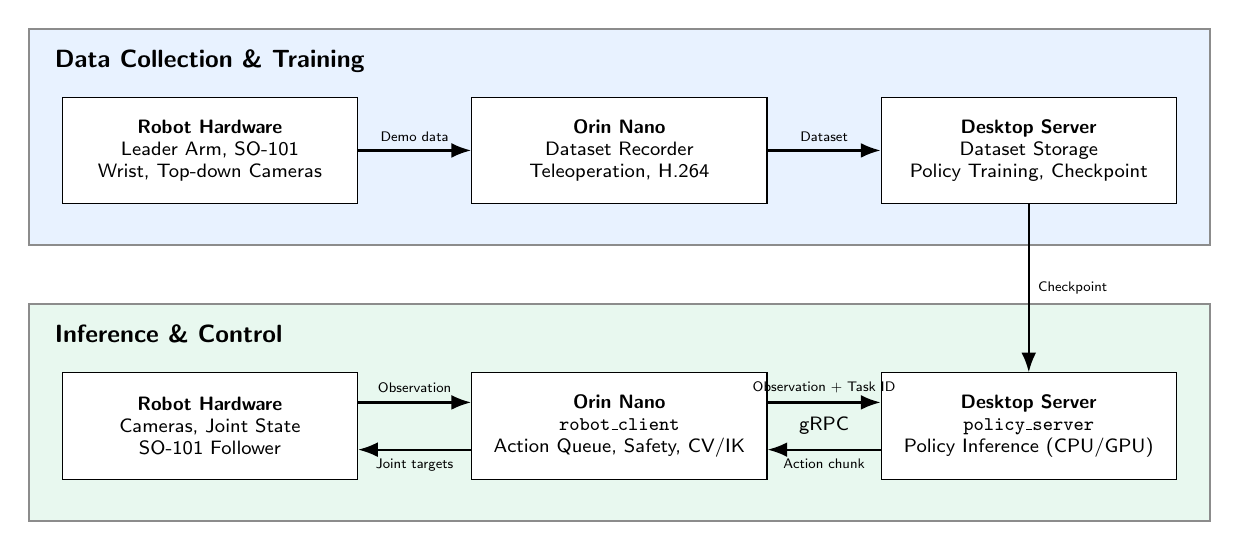
\begin{tikzpicture}[
    phase/.style={rectangle, draw=black!45, thick, minimum width=15.0cm, minimum height=2.75cm},
    phasetitle/.style={font=\sffamily\bfseries\small, anchor=north west},
    host/.style={rectangle, draw=black, fill=white, align=center, minimum width=3.75cm, minimum height=1.35cm, inner sep=3pt, font=\sffamily\scriptsize},
    dataflow/.style={-{Latex[length=2.5mm]}, thick},
    flowlabel/.style={font=\sffamily\tiny, align=center, inner sep=1pt}
]
\node[phase,fill=boxblue] (offline) at (5.2,1.75) {};
\node[phase,fill=boxgreen] (online) at (5.2,-1.75) {};
\node[phasetitle] at ([xshift=0.22cm,yshift=-0.16cm]offline.north west) {Data Collection \& Training};
\node[phasetitle] at ([xshift=0.22cm,yshift=-0.16cm]online.north west) {Inference \& Control};

\node[host] (collectrobot) at (0,1.58) {\textbf{Robot Hardware}\\Leader Arm, SO-101\\Wrist, Top-down Cameras};
\node[host] (recorder) at (5.2,1.58) {\textbf{Orin Nano}\\Dataset Recorder\\Teleoperation, H.264};
\node[host] (trainer) at (10.4,1.58) {\textbf{Desktop Server}\\Dataset Storage\\Policy Training, Checkpoint};

\node[host] (runtimeRobot) at (0,-1.92) {\textbf{Robot Hardware}\\Cameras, Joint State\\SO-101 Follower};
\node[host] (client) at (5.2,-1.92) {\textbf{Orin Nano}\\\texttt{robot\_client}\\Action Queue, Safety, CV/IK};
\node[host] (server) at (10.4,-1.92) {\textbf{Desktop Server}\\\texttt{policy\_server}\\Policy Inference (CPU/GPU)};

\draw[dataflow] (collectrobot.east) --
    node[flowlabel,above,yshift=2pt] {Demo data} (recorder.west);
\draw[dataflow] (recorder.east) --
    node[flowlabel,above,yshift=2pt] {Dataset} (trainer.west);
\draw[dataflow] (trainer.south) --
    node[flowlabel,right,xshift=2pt] {Checkpoint} (server.north);

\draw[dataflow] ([yshift=0.30cm]runtimeRobot.east) --
    node[flowlabel,above,yshift=2pt] {Observation} ([yshift=0.30cm]client.west);
\draw[dataflow] ([yshift=-0.30cm]client.west) --
    node[flowlabel,below,yshift=-2pt] {Joint targets} ([yshift=-0.30cm]runtimeRobot.east);
\draw[dataflow] ([yshift=0.30cm]client.east) --
    node[flowlabel,above,yshift=2pt] {Observation + Task ID} ([yshift=0.30cm]server.west);
\draw[dataflow] ([yshift=-0.30cm]server.west) --
    node[flowlabel,below,yshift=-2pt] {Action chunk} ([yshift=-0.30cm]client.east);
\node[font=\sffamily\scriptsize,inner sep=1pt] at (7.8,-1.92) {gRPC};
\end{tikzpicture}%
}
\caption{데이터 수집 및 학습과 추론 및 제어를 구분한 전체 시스템 아키텍처}
\label{fig:system-architecture-updated}
\end{figure}

\section{단일 모델 시스템 후보별 구조}

Task ID 기반 ACT는 기존 ACT\cite{zhao2023act}의 영상 및 관절 상태 입력에 1차와 2차 미션을 구분하는 이산 Task ID를 추가하는 설계 후보이다. Task ID는 각 미션에 부여한 임의의 식별자이며 자연어 명령이나 언어 임베딩은 사용하지 않는다. 기존 ACT의 구조와 액션 청크 제어를 유지하면서, 하나의 가중치가 Task ID에 따라 두 미션의 행동을 구분하도록 학습한다.

SmolVLA는 SmolVLM2 기반의 비전-언어 백본 위에 로봇 행동을 예측하는 action expert가 결합된 구조로, 영상과 관절 상태에 더해 \textbf{언어 명령}을 입력으로 받는다. 사전학습 가중치(\texttt{smolvla\_base})를 파인튜닝하며, 주요 학습 설정은 카메라 2개 매핑(\texttt{camera1/2}), 태스크 언어 지시(\texttt{-{}-task}), 액션 청크 길이 50이다.

\begin{figure}[htbp]
\centering
\resizebox{0.96\textwidth}{!}{%
\begin{tikzpicture}[
    input/.style={rectangle, draw=black, fill=boxgray, align=center, minimum width=2.8cm, minimum height=0.85cm, font=\sffamily\scriptsize},
    backbone/.style={rectangle, draw=black, thick, fill=boxblue, align=center, minimum width=3.0cm, minimum height=1.05cm, font=\sffamily\scriptsize},
    expert/.style={rectangle, draw=black, thick, fill=boxgreen, align=center, minimum width=3.0cm, minimum height=1.05cm, font=\sffamily\scriptsize},
    arrow/.style={-{Latex[length=3mm]}, thick}
]
\node[input] (wrist) at (0,1.8) {Wrist Camera\\근접 파지 뷰};
\node[input] (top) at (0,0.6) {Top-down Camera\\전역 뷰};
\node[input] (lang) at (0,-0.6) {Language Command\\``모아라'' / ``쌓아라''};
\node[input] (joint) at (0,-1.8) {Joint State\\관절 상태};
\node[backbone] (encoder) at (4.1,0.6) {VLM Backbone\\SmolVLM2};
\node[expert] (act) at (8.0,0.0) {Action Expert\\Flow Matching};
\node[expert] (action) at (12.0,0.0) {Action Chunk\\$50 \times 6$ joint targets};

\draw[arrow] (wrist) -- (encoder);
\draw[arrow] (top) -- (encoder);
\draw[arrow] (lang) -- (encoder);
\draw[arrow] (encoder) -- (act);
\draw[arrow] (joint.east) -- ++(1.1,0) -| (act.south);
\draw[arrow] (act) -- (action);
\end{tikzpicture}
}
\caption{SmolVLA 모방학습 정책 구조. 언어 명령에 따라 단일 모델이 이동과 적재 태스크를 구분하도록 학습한다.}
\label{fig:policy_structure_smolvla}
\end{figure}

하이브리드 ACT--CV/IK는 학습이 필요한 비정형 접촉 동작과 기하학적으로 표현할 수 있는 배치 동작을 분리한다. ACT는 임의의 초기 위치에서 블록에 접근하여 파지하고 고정 retreat 자세까지 들어 올린다. 제어기는 그리퍼 관절의 닫힘 상태, 순기구학(FK)으로 계산한 말단 높이와 retreat 자세 도달 여부를 함께 확인한 후 CV/IK 단계로 전환한다. 파지가 확인되지 않으면 초기 자세로 복귀하여 ACT를 다시 실행한다. 전환 오검출을 줄이기 위해 모든 관절이 목표 자세의 허용 오차 안에 일정 시간 연속으로 머무는 조건을 사용할 예정이며, 허용 오차와 유지 시간은 실험으로 결정한다.

탑다운 영상에서는 OpenCV의 HSV 색상 임계값, 모폴로지 연산과 윤곽선 검출을 사용하며 신경망 기반 객체 검출기는 사용하지 않는다\cite{opencv}. 화소 좌표는 사전 보정한 homography로 테이블 좌표계로 변환한다. 1차 미션은 20cm $\times$ 10cm 영역 안에 블록 크기와 여유 간격을 고려한 5개 비중첩 배치 슬롯을 정의하고, CV로 점유 상태를 확인하여 빈 슬롯을 목표 $x,y$로 선택한다. 이는 모든 블록을 영역 중심에 놓아 적재되는 것을 방지하기 위한 설계이다. 2차 미션은 기존 탑 상단 블록의 중심을 목표 $x,y$로 사용한다. 기존 적재 블록 수를 $n$, 블록 높이를 $h=2$cm로 두면 2차 미션의 해제 높이는 $z_{\mathrm{release}}(n)=z_{\mathrm{release}}(0)+nh$로 계산한다. IK는 현재 관절 상태에서 안전 상승, 수평 이동, 하강, 그리퍼 해제 웨이포인트를 순차적으로 생성한다.

하이브리드 방식은 정밀한 배치를 명시적으로 제어하고 기하학적으로 표현 가능한 새 과제를 재학습 없이 추가할 수 있다는 장점이 있다. 반면 조명과 배경 변화에 따른 색상 분할 실패, homography 보정 오차, 기구학 모델 오차, ACT와 CV/IK 사이의 전환 실패가 누적될 수 있다. 또한 새 과제가 모두 기하학적 규칙으로 표현된다고 보장할 수 없으므로, 이 후보의 확장성은 Task ID 기반 ACT와 SmolVLA의 학습 기반 확장성과 구분해 평가한다.

\begin{figure}[htbp]
\centering
\resizebox{0.78\textwidth}{!}{%
\begin{tikzpicture}[
    node distance=0.65cm and 1.5cm,
    terminal/.style={rectangle, rounded corners=4pt, draw=black, thick, fill=white, align=center, minimum width=3.4cm, minimum height=0.85cm, font=\sffamily\scriptsize},
    policy/.style={rectangle, draw=black, thick, fill=boxblue, align=center, minimum width=3.4cm, minimum height=1.0cm, font=\sffamily\scriptsize},
    process/.style={rectangle, draw=black, thick, fill=boxgray, align=center, minimum width=3.4cm, minimum height=1.0cm, font=\sffamily\scriptsize},
    target/.style={rectangle, draw=black, thick, fill=white, align=center, minimum width=3.3cm, minimum height=0.95cm, font=\sffamily\scriptsize},
    control/.style={rectangle, draw=black, thick, fill=boxgreen, align=center, minimum width=3.4cm, minimum height=1.0cm, font=\sffamily\scriptsize},
    decision/.style={diamond, draw=black, thick, fill=boxgray, aspect=2.1, align=center, inner sep=1.5pt, font=\sffamily\scriptsize},
    harrow/.style={-{Latex[length=3mm]}, thick},
    branch/.style={font=\sffamily\scriptsize, inner sep=1pt}
]
\node[terminal] (start) {Start\\Task 선택 및 초기 상태 관측};
\node[policy,below=of start] (act) {ACT (single neural model)\\접근 $\rightarrow$ 파지 $\rightarrow$ 들기};
\node[decision,below=of act] (verify) {파지 성공?};
\node[process,right=of verify] (retry) {Home 자세 복귀\\ACT 재시도};
\node[process,below=of verify] (cv) {Traditional CV\\HSV, morphology, contour};
\node[decision,below=of cv] (mission) {Mission?};
\node[target,below left=0.8cm and 0.9cm of mission] (taskone) {Task 1\\빈 배치 슬롯};
\node[target,below right=0.8cm and 0.9cm of mission] (tasktwo) {Task 2\\탑 중심과 높이};
\node[control,below=2.7cm of mission] (ik) {Homography + IK\\이동};
\node[control,below=of ik] (release) {Place};

\draw[harrow] (start) -- (act);
\draw[harrow] (act) -- (verify);
\draw[harrow] (verify) -- node[branch,left] {Yes} (cv);
\draw[harrow] (verify) -- node[branch,above] {No} (retry);
\draw[harrow] (retry.north) |- (act.east);
\draw[harrow] (cv) -- (mission);
\draw[harrow] (mission) -- node[branch,above left] {Task 1} (taskone);
\draw[harrow] (mission) -- node[branch,above right] {Task 2} (tasktwo);
\draw[harrow] (taskone.south) |- (ik.west);
\draw[harrow] (tasktwo.south) |- (ik.east);
\draw[harrow] (ik) -- (release);
\end{tikzpicture}%
}
\caption{하이브리드 ACT--CV/IK 제어 흐름. 파지 실패 시 ACT를 재시도하고, 파지 성공 후 미션별 목표를 선택해 CV와 IK로 배치한다.}
\label{fig:hybrid-act-cv-ik}
\end{figure}

\section{정량 평가 및 rollout 기록 체계}

과제 공지의 공식 평가는 제한 시간 안에 성공한 블록 수와 전체 완료 시간을 기준으로 한다. 이와 별도로 정책의 실패 단계를 분석하고 학습 조건별 성능을 비교하기 위해 팀 공통 평가 기록 양식을 마련하였다. 이 양식은 파지, 배치, 적재와 유지 성공 여부를 각 rollout마다 1 또는 0으로 기록하며, 공식 채점 결과와 모델 개선을 위한 내부 진단 지표를 다음과 같이 구분한다.

\begin{longtable}{@{}p{0.26\linewidth}p{0.50\linewidth}p{0.18\linewidth}@{}}
\toprule
평가 지표 & 평가 기준 & 적용 범위 \\
\midrule
\endhead
\multicolumn{3}{@{}l}{\textbf{공식 평가 지표}} \\
1차 수행 결과 & 3분 내 지정 영역에 놓인 블록 수, 5개 완료 시 소요 시간 & 1차 (이동) \\
2차 수행 결과 & 5분 내 안정적으로 쌓은 블록 수, 5개 완료 시 소요 시간 & 2차 (적재) \\
\midrule
\multicolumn{3}{@{}l}{\textbf{내부 분석 지표}} \\
파지 성공 여부 & 그리퍼가 블록을 집어 들어 올렸는지 1 또는 0으로 기록 & 공통 \\
안착 성공 여부 & 블록을 지정 영역 안에 쌓지 않고 놓았는지 기록 & 1차 (이동) \\
적재 성공 여부 & 기존 블록 위에 무너뜨리지 않고 쌓았는지 기록 & 2차 (적재) \\
5초 유지 여부 & 블록을 놓은 뒤 5초 이상 안정적으로 유지됐는지 기록 & 2차 (최종 판정) \\
전체 성공과 실패 단계 & 최종 성공 여부와 실패 지점(grasp, transport, place, hold) 기록 & 공통 \\
완료 시간 & rollout 시작부터 완료까지 걸린 시간(초) 기록 & 공통 \\
\bottomrule
\end{longtable}

공통 프로토콜은 조건당 rollout 10회 수행, 조건 내 초기 위치 세트 고정, 한 번에 하나의 조건만 변경, 매 rollout의 성공 여부와 실패 단계 기록의 네 원칙으로 구성된다. 조건별 성공률은 전체 성공 횟수를 10으로 나누어 계산하며, 정책 후보를 비교할 때에는 같은 초기 위치 세트를 사용한다. 변경 조건은 데이터 양, 카메라 높이, 액션 청크와 조명 등으로 기록한다.

하이브리드 ACT--CV/IK 후보에는 파지 정책에서 규칙 제어로의 전환 성공 여부, CV 목표 좌표 오차와 IK 배치 오차가 추가로 필요하다. 이 세 항목은 하이브리드 구현을 진단하기 위한 후보 지표이며 현재 팀 공통 평가 기록 양식에는 포함되지 않았다. 구현 후 측정 방법을 확정하고 팀 합의를 거쳐 양식에 추가한다. 네트워크 지연, 추론 시간과 액션 큐 고갈 여부는 task 성공률과 분리된 시스템 성능 항목으로 기록한다.

% =====================================================================
\chapter{갱신된 과제 추진 계획}

전체 일정은 환경 구축이 본격화된 7월 1주부터 결과물 업로드까지로 구성한다. 보고 시점인 7월 17일까지 듀얼 카메라와 텔레오퍼레이션 환경, 원격 추론 구조, 초기 ACT 및 SmolVLA 학습을 완료했으며, 이후에는 세 정책 후보를 동일한 초기 위치와 평가 기준으로 비교하고 선정한 후보를 두 미션에 통합한다. 데이터 수집량은 약 300개와 같은 고정 목표로 두지 않고, 반복 평가에서 확인된 실패 위치와 동작 구간을 중심으로 보강한다. 7월 4주부터 8월 2주까지 3주간 후보별 정량 비교를 수행하고 8월 2주에 최종 후보를 선정한 뒤, 9월 2주까지 1차 및 2차 미션 통합, 5초 적재 유지, Docker 평가 서버 호환성 검증을 완료한다. 최종보고서와 최종평가표는 9월 18일까지 제출하고, 이후 모델과 실행 환경을 동결하여 9월 30일 또는 10월 1일 발표심사를 준비한다.

강화학습 기반 ManiSkill sim2real은 핵심 미션과 배포 검증을 계획보다 일찍 완료한 경우에만 수행하는 선택 과제로 두며, 아래 핵심 일정에는 포함하지 않는다.

\begingroup
\scriptsize
\renewcommand{\arraystretch}{1.0}
\setlength{\tabcolsep}{2pt}
\begin{longtable}{@{}p{0.41\linewidth}*{16}{>{\centering\arraybackslash}p{0.027\linewidth}}@{}}
\toprule
업무 & \multicolumn{4}{c}{7월} & \multicolumn{4}{c}{8월} & \multicolumn{4}{c}{9월} & \multicolumn{4}{c}{10월} \\
\cmidrule(lr){2-5}\cmidrule(lr){6-9}\cmidrule(lr){10-13}\cmidrule(lr){14-17}
 & 1 & 2 & 3 & 4 & 1 & 2 & 3 & 4 & 1 & 2 & 3 & 4 & 1 & 2 & 3 & 4 \\
\midrule
\endhead
듀얼 카메라, 텔레오퍼레이션과 원격 추론 환경 구축 & \ganttdone & \ganttdone & & & & & & & & & & & & & & \\
초기 데이터 수집과 ACT, SmolVLA 기준 학습 & & \ganttdone & \ganttdone & & & & & & & & & & & & & \\
기준 성능 기록 및 공통 파지 데이터 보강 & & & \ganttdone & \ganttbar & \ganttbar & & & & & & & & & & & \\
Task ID 기반 ACT 구현 및 다중 미션 학습 & & & & \ganttbar & \ganttbar & \ganttbar & & & & & & & & & & \\
SmolVLA 다중 미션 데이터 구성 및 학습 & & & & \ganttbar & \ganttbar & \ganttbar & & & & & & & & & & \\
CV 좌표 보정, Homography와 IK 구현 및 통합 & & & \ganttbar & \ganttbar & \ganttbar & \ganttbar & & & & & & & & & & \\
세 정책 후보 동일 조건 반복 평가 & & & & \ganttbar & \ganttbar & \ganttbar & & & & & & & & & & \\
최종 정책 후보 선정 & & & & & & \ganttbar & & & & & & & & & & \\
1차 및 2차 미션 통합과 5초 유지 튜닝 & & & & & & & \ganttbar & \ganttbar & \ganttbar & & & & & & & \\
최종 반복 평가 및 실패 데이터 보강 & & & & & & & & & \ganttbar & \ganttbar & & & & & & \\
Docker 패키징 및 평가 서버 호환성 검증 & & & & & & & \ganttbar & \ganttbar & \ganttbar & \ganttbar & & & & & & \\
\textbf{최종보고서 및 최종평가표 제출 (9/18)} & & & & & & & & & & & \ganttmilestone & & & & & \\
모델 동결, 평가 리허설과 발표 준비 & & & & & & & & & & & \ganttbar & \ganttbar & & & & \\
\textbf{졸업과제 발표심사 (9/30 또는 10/1)} & & & & & & & & & & & & \multicolumn{2}{c}{\ganttmilestone} & & & \\
결과물 업로드 (10월 중순) & & & & & & & & & & & & & & \ganttmilestone & & \\
\midrule
\multicolumn{17}{@{}l}{표시: 검은 막대는 완료, 회색 막대는 이후 계획, 삼각형은 공식 일정} \\
\bottomrule
\end{longtable}
\endgroup

% =====================================================================
\chapter{구성원별 진척도}

\begin{longtable}{p{0.16\linewidth}p{0.56\linewidth}p{0.20\linewidth}}
\toprule
이름 & 담당 및 수행 내용 & 진척도 \\
\midrule
\endhead
윤민석 & SO-101 제어와 캘리브레이션, \texttt{robot\_client} 및 Action 검증 안전 로직. 파랑과 기본 블록 데이터 수집, SmolVLA 학습 및 rollout 테스트, 카메라와 테이프 환경 정비, 실제 로봇 통합 검증. & 로봇 제어, 데이터와 학습 검증 완료 \\
이동근 & 프로젝트 초기 셋업과 리더암--팔로워암 제어 환경, 듀얼 카메라 웹 뷰어 및 동기화, 데스크톱과 Orin Nano를 연결하는 gRPC 기반 원격 추론 환경 구축. 초록과 노랑 블록 및 단일 블록 pick-and-place 데이터 수집, ACT와 SmolVLA 학습 비교, ACT 청크 옵션 튜닝. & 데이터, 학습과 원격 추론 환경 구축 완료 \\
김주환 & SmolVLA 정책 설계와 학습, 하이퍼파라미터와 학습 로그 분석, 평가 지표 정의, Docker 기반 \texttt{policy\_server} 배포 절차 검토. 정량 평가 체계 신규 정의 및 기록 템플릿 배포, 캘리브레이션 절차 점검. & 평가 체계 완료 / Docker 및 로그 분석 착수 예정 \\
전체 팀원 & 실제 로봇 통합 테스트, 실패 사례 분석과 데이터 보강, 보고서 및 발표 준비. & 진행 중 \\
\bottomrule
\end{longtable}

공통적으로 데이터 수집--학습--추론 파이프라인이 반복 가능한 형태로 정착되었고 서버 통신도 해결되어 rollout 검증이 가능해졌다. 현재 팀 전체의 최우선 과제는 위치와 색상 다양성을 확대하고 CV 좌표 보정과 IK 배치 제어를 구성한 뒤, 세 후보의 성공률과 운용 비용을 정량 비교하는 것이다.

% =====================================================================
\chapter{보고 시점까지의 과제 수행 내용 및 중간 결과}

\section{실험 환경 및 하드웨어 셋업}

리더암 텔레오퍼레이션으로 시연 데이터를 수집하고, 팔로워암(SO-ARM101)이 이를 실행하는 환경을 구축하였다. 작업 공간 바닥은 체스판 패턴을 사용하고, 지정구역은 내부 규격 20$\times$10cm, 로봇 끝 기준 25cm 위치 조건에 맞춰 빨간색 테이프로 표시하였다. 탑다운 카메라는 작업 공간을 관측하도록 배치하였다. 공식 평가에서는 5개 블록이 모두 넓은 면을 바닥으로 향한 채 지정구역 밖의 무작위 위치에 놓이고, 서로 맞닿아 배치될 수 있다. 두 미션은 별도로 진행되며 미션마다 블록이 다시 배치된다.

초기 테스트 이후 인식 성능 개선을 위해 실험 환경을 일부 정비하였다. 첫째, 탑다운 카메라의 위치를 기존보다 높여 경기장 전체가 관측되도록 각도를 조정하였다. 둘째, 지정구역 표시 테이프를 내부 규격과 로봇으로부터의 거리 조건에 맞게 다시 부착하였다(그림~\ref{fig:env-improve}). 이러한 정비로 관측 범위 확대와 시각적 기준 정렬을 통한 인식 성능 향상을 기대하고 있다. 다만 카메라와 테이프 배치가 변경되었으므로, 기존 에피소드는 새 환경 기준으로 재수집이 필요하다.

\begin{figure}[!htbp]
\centering
\begin{subfigure}[b]{0.48\textwidth}
\centering
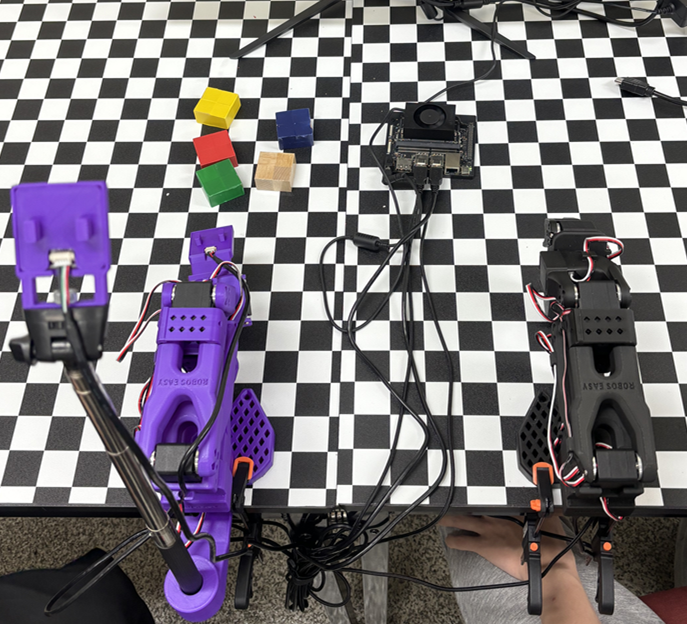
\includegraphics[width=\linewidth]{setup_front.png}
\caption{로봇과 카메라 셋업}
\label{fig:setup}
\end{subfigure}
\hfill
\begin{subfigure}[b]{0.34\textwidth}
\centering
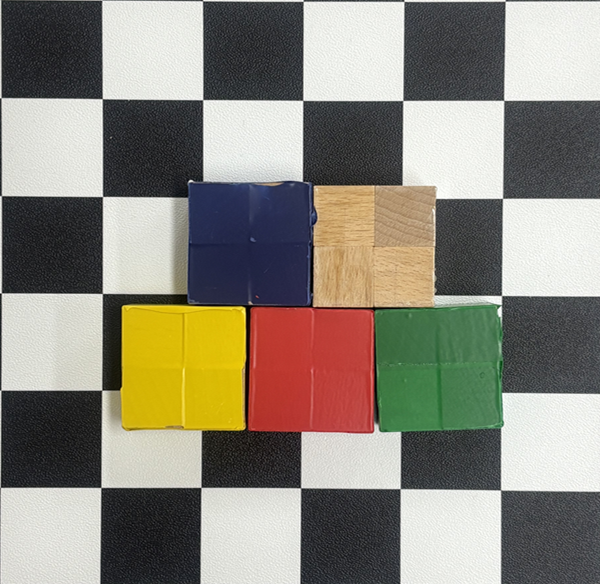
\includegraphics[width=\linewidth]{blocks5.png}
\caption{과제 대상 블록 5개}
\label{fig:blocks}
\end{subfigure}
\caption{실험 환경 및 대상 물체}
\label{fig:env}
\end{figure}

\begin{figure}[htbp]
\centering
\begin{subfigure}{0.44\textwidth}
\centering
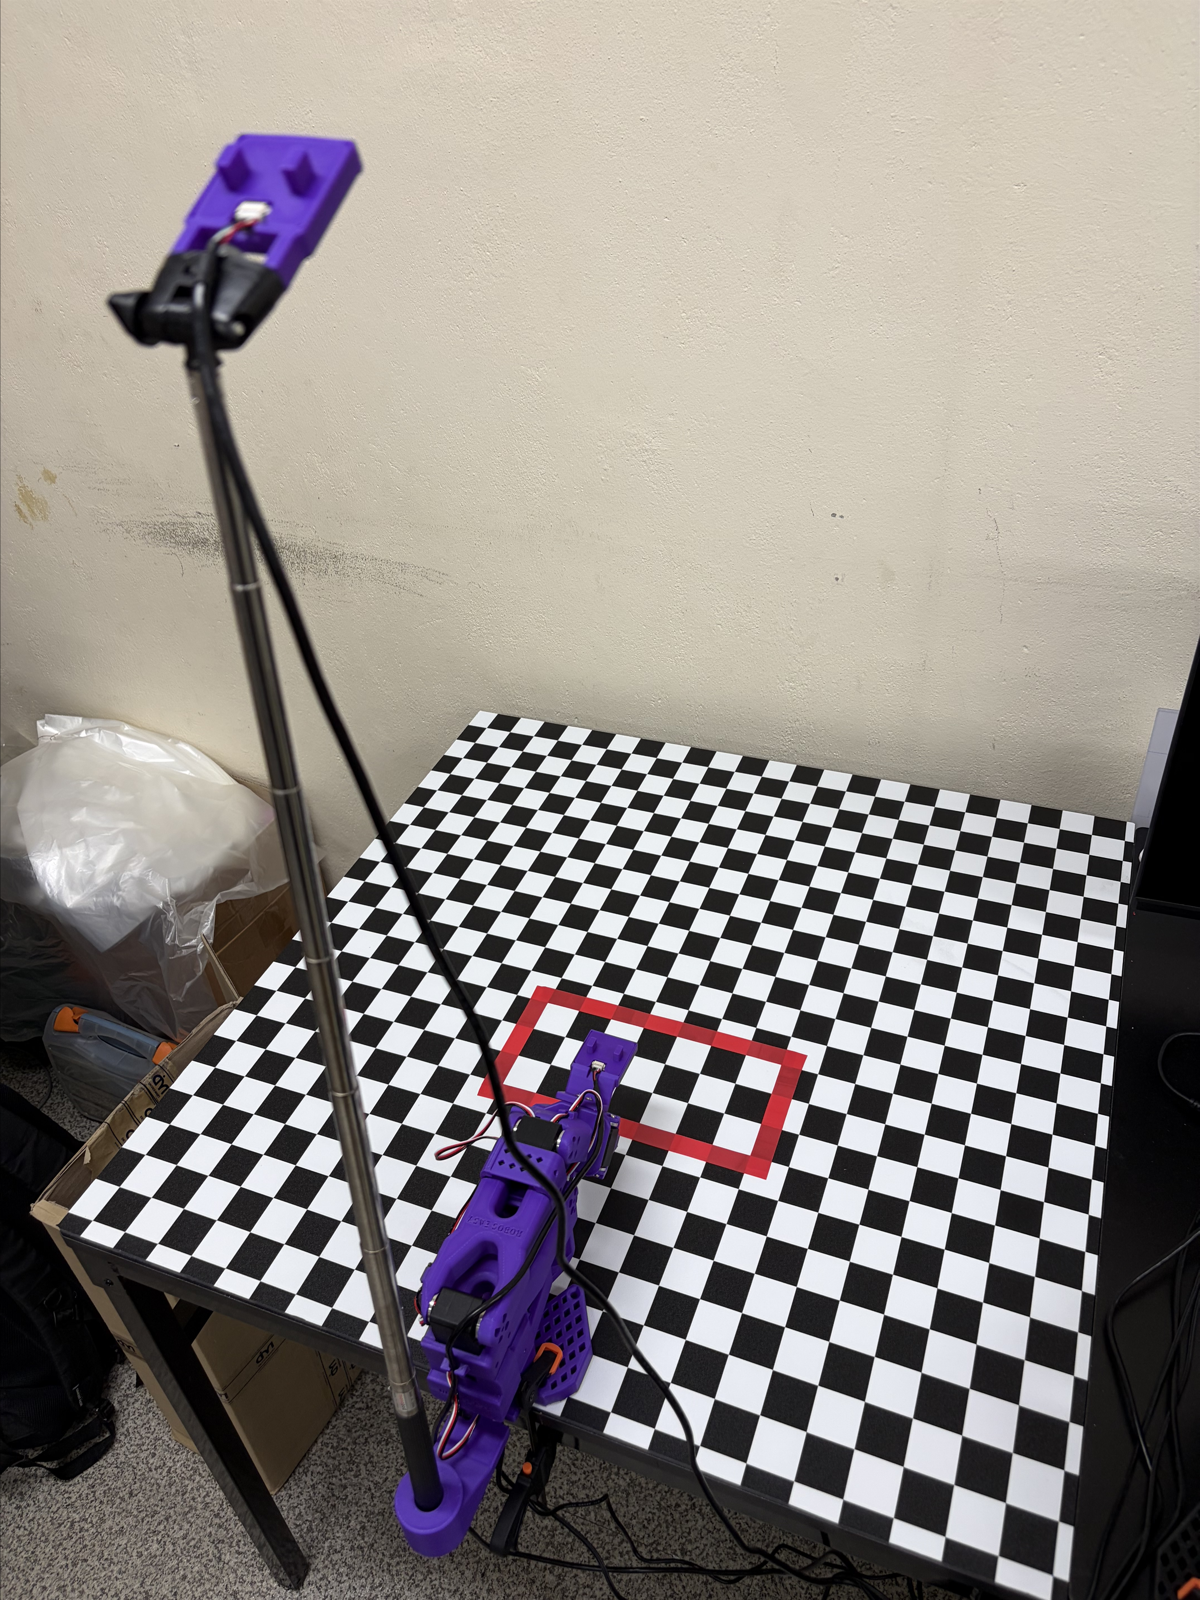
\includegraphics[height=6.2cm]{camera_high.png}
\caption{경기장 전체 관측을 위한 탑다운 카메라 높이 조정}
\label{fig:camera-high}
\end{subfigure}
\hfill
\begin{subfigure}{0.44\textwidth}
\centering
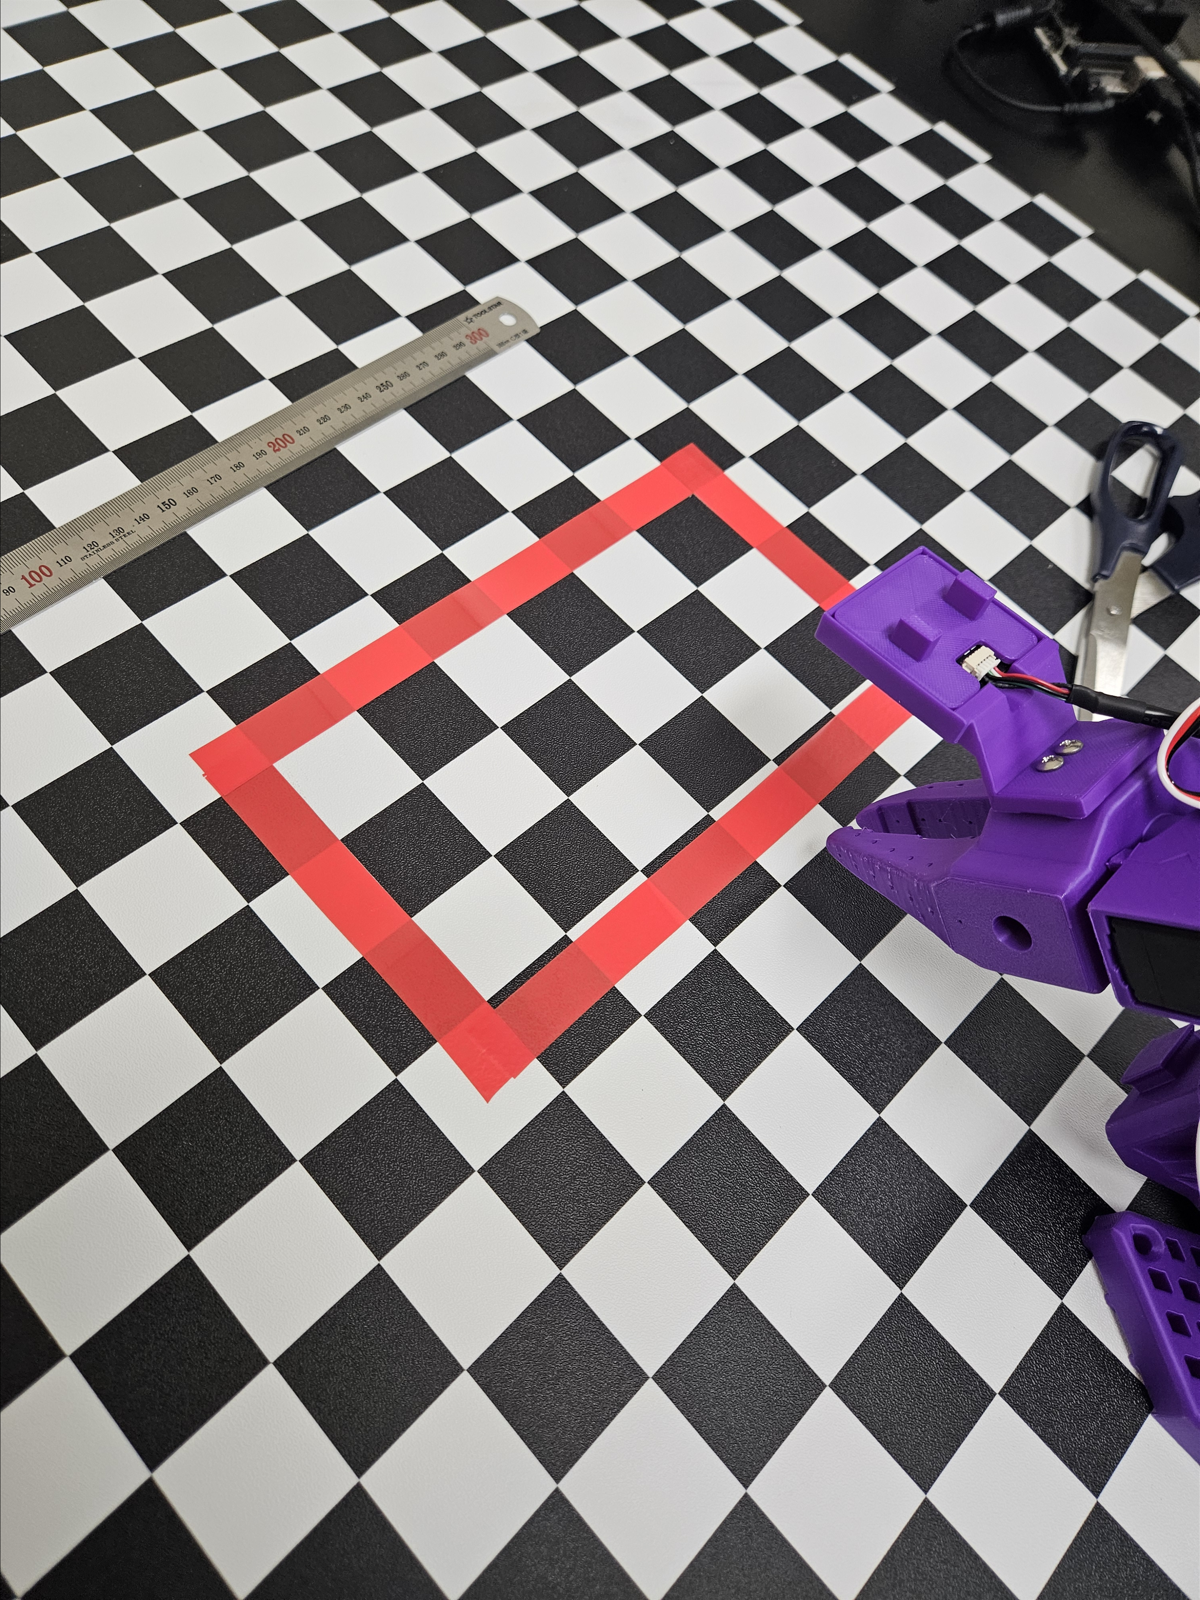
\includegraphics[height=6.2cm]{tape_measure.png}
\caption{격자 라인 정렬 및 규격 실측을 통한 테이프 재부착}
\label{fig:tape-measure}
\end{subfigure}
\caption{인식 성능 개선을 위한 실험 환경 정비}
\label{fig:env-improve}
\end{figure}


\FloatBarrier
\section{텔레오퍼레이션 데이터 수집 및 캘리브레이션}

데이터 수집 전 리더암과 팔로워암을 각각 캘리브레이션하고 텔레오퍼레이션 동작을 확인하였다. 리더암으로 팔로워암을 조작하면서 손목 카메라와 탑다운 카메라 영상, 관절 상태와 행동을 동기화하여 LeRobotDataset 형식으로 저장하였다. 그림~\ref{fig:collect}(a)는 리더암으로 팔로워암을 조작하며 시연을 수집하는 상단 시점이고, 그림~\ref{fig:collect}(b)는 캘리브레이션 후 지정구역을 기준으로 로봇의 배치 상태를 확인하는 모습이다. 초록과 노랑 데이터셋은 색상별로 수집한 뒤 51개 에피소드의 통합 데이터셋으로 병합하였으며, 색상별 데이터셋과 통합 데이터셋을 Hugging Face에 업로드하였다. 또한 에피소드 종료 후 인코딩 대기 시간을 줄이기 위해 영상 코덱을 AV1에서 H.264로 변경하였다.

후속 공통 파지 데이터는 여러 블록을 무작위로 배치하고, 고정 home 자세에서 접근, 정렬, 파지와 들어 올리기를 수행한 뒤 고정 retreat 자세에서 종료하는 형식으로 수집할 계획이다. 접근과 정렬 구간은 감속하고 블록 위에서 1--2초간 수직 자세를 유지한다. 에피소드 사이의 reset 시간은 약 4초로 설정하고 H.264 인코딩을 계속 사용한다.

\begin{figure}[htbp]
\centering
\begin{subfigure}[b]{0.48\textwidth}
\centering
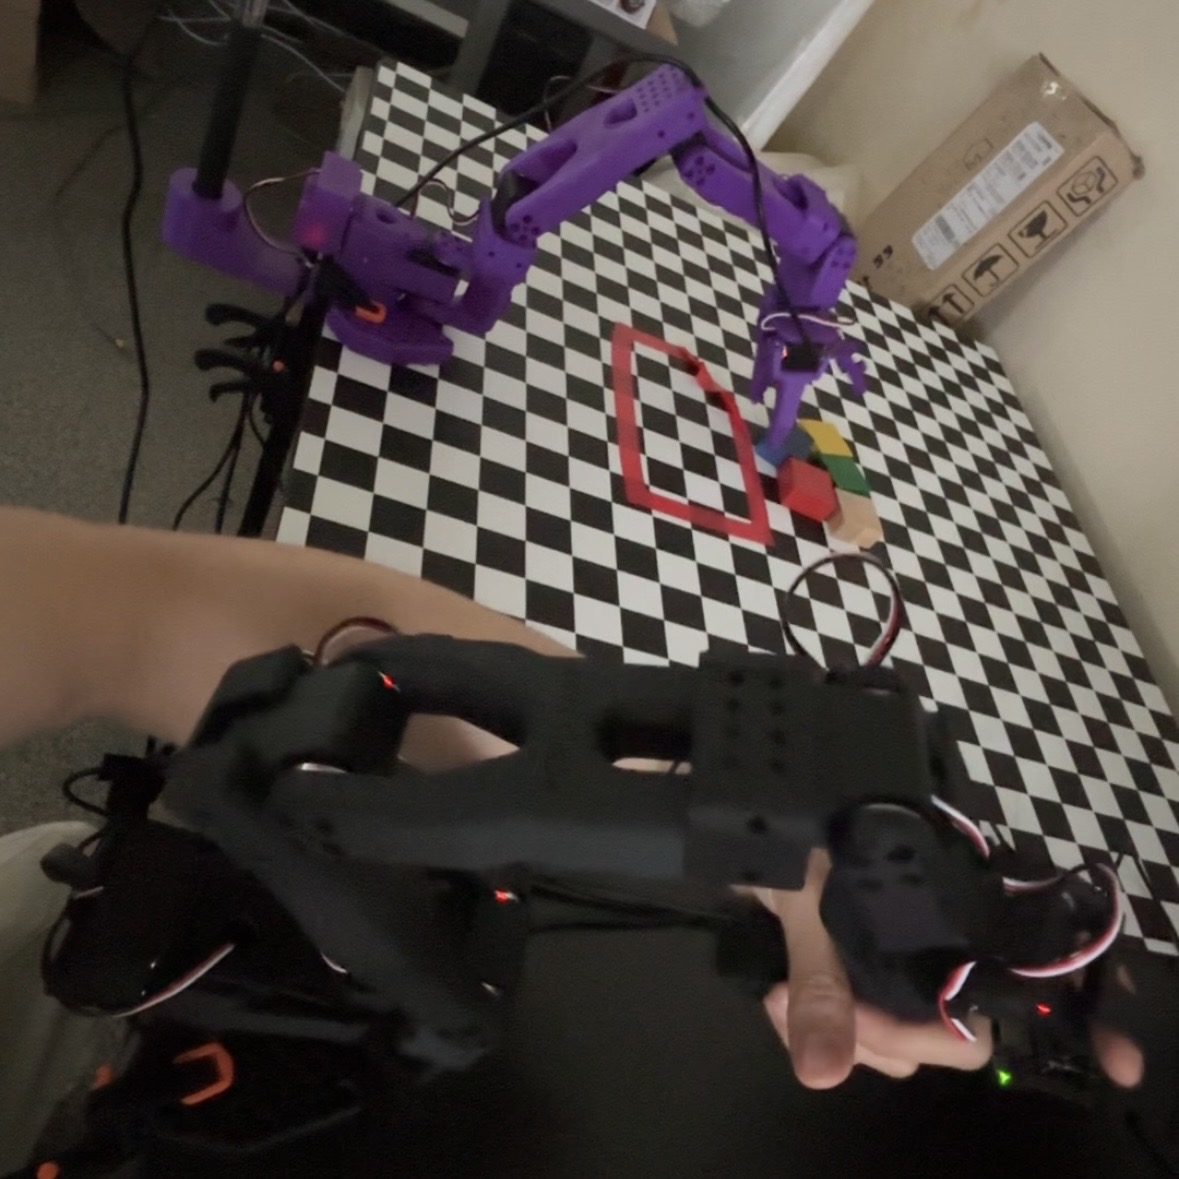
\includegraphics[width=\linewidth]{teleop_topview.png}
\caption{리더암 텔레오퍼레이션(상단 시점)}
\label{fig:teleop}
\end{subfigure}
\hfill
\begin{subfigure}[b]{0.48\textwidth}
\centering
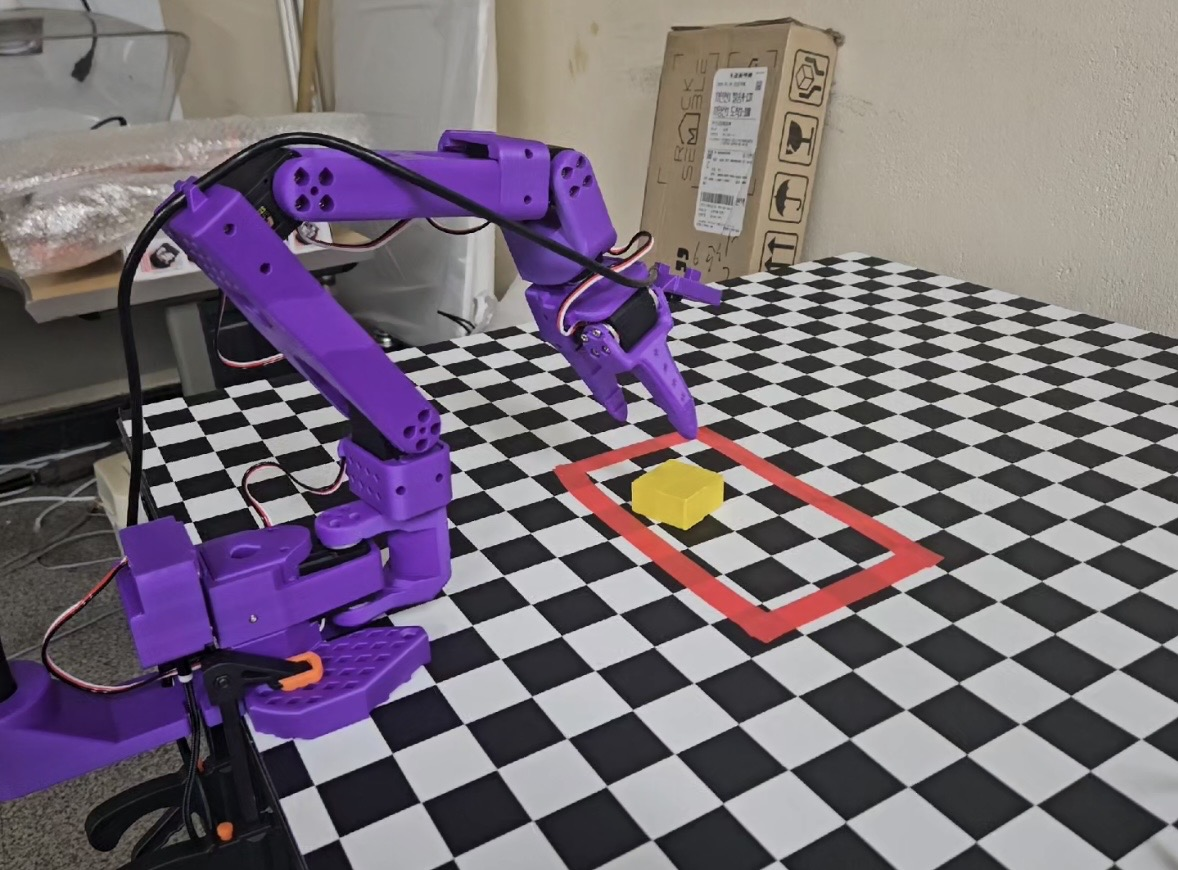
\includegraphics[width=\linewidth]{calibration.png}
\caption{캘리브레이션 및 지정구역 배치 확인}
\label{fig:calib}
\end{subfigure}
\caption{데이터 수집 및 캘리브레이션 과정}
\label{fig:collect}
\end{figure}

\FloatBarrier
\section{데이터셋 구축 현황}

색깔별 블록 시연 데이터를 순차적으로 수집하여 현재까지 총 112개 에피소드를 확보하였다. 빨간색 블록은 경계선 방향 이동 현상의 원인이 확인될 때까지 수집을 보류하였다. 현재 계획상 약 300개 에피소드를 잠정 목표로 두되, 에피소드 수를 일률적으로 늘리기보다 실패 구간과 초기 위치 다양성을 집중 보강하고 정량 평가 결과에 따라 목표량을 조정한다.

\begin{longtable}{p{0.18\linewidth}p{0.14\linewidth}p{0.14\linewidth}p{0.14\linewidth}p{0.14\linewidth}}
\toprule
색상 & 초록 & 노랑 & 파랑 & 기본(default) \\
\midrule
\endhead
에피소드 & 31 & 20 & 31 & 30 \\
\bottomrule
\end{longtable}

\section{모델 학습 및 중간 결과}

초록 31개와 노랑 20개의 단일 블록 pick-and-place 데이터(총 51 에피소드)를 병합하여 \texttt{smolvla\_base}를 파인튜닝(8{,}000 스텝)한 첫 모델을 확보하였고, 이후 파랑과 기본 데이터를 추가하여 재학습을 진행하였다. 학습된 정책을 데스크톱 GPU에서 실행하여 블록 파지와 이동 동작을 확인하였다.

\textbf{SmolVLA 테스트.} 색깔별 데이터로 학습한 SmolVLA 정책을 실제 로봇에서 실행한 결과, 팔로워암이 목표 위치까지는 이동하였으나 파지가 제대로 이루어지지 않았다. 파지 실패의 원인으로는 시연 데이터의 양과 다양성 부족과 함께, 녹화 시 동작 속도가 빨라 접근 정렬이 부정확했던 점을 추정하고 있다. 현 결과는 제한된 초기 rollout에서 관찰한 정성 결과이며, 동일 초기 위치에서 반복한 성공 횟수는 후속 평가에서 기록한다.

\textbf{일반 ACT 선행 테스트.} Task ID 기반 ACT를 구성하기 전에 ACT 기본 정책의 제어 성능을 검증하였다. 블록 위치를 기준 위치에서 $\pm 3$cm 범위로 변화시키며 약 30개 에피소드를 수집하고 학습하였다. 그림~\ref{fig:result}는 일반 ACT 정책이 노란 블록을 파지하여 들어 올리는 순간이다. 제한된 초기 rollout에서 지정구역 이동 성공률은 튜닝 전 약 15\%, 액션 청크 갱신과 혼합 옵션 조정 후 약 60\%로 관찰되었다. 현재 수치는 시험 횟수와 성공 횟수를 별도로 기록하기 전에 얻은 잠정값이므로 후보 간 정량 비교값으로 사용하지 않는다. 다만 청크 옵션 조정 후 동작 끊김이 줄었고, 한 번에 올바른 파지 자세를 잡지 못한 경우의 복구(recovery) 능력은 여전히 부족했다. 이 결과는 ACT 계열의 액션 청크 제어가 본 시스템에서 동작함을 보이며, Task ID 기반 ACT의 기반이자 하이브리드 ACT--CV/IK의 공통 파지 단계로 활용할 수 있다는 실험적 근거가 된다.

현 단계에서는 위치 변화가 작은 조건에서 일반 ACT가 SmolVLA보다 안정적인 성능을 보였다. 다만 일반 ACT는 아직 두 미션을 전체적으로 구분하는 정책이 아니고, 하이브리드 후보의 CV/IK 배치도 구현 전이므로 이 결과만으로 최종 방식을 판단하지 않는다. 다음 단계에서 동일한 환경으로 Task ID 기반 ACT, SmolVLA, 하이브리드 ACT--CV/IK를 평가하고 미션별 성공률과 실행 시간을 비교한다.

\begin{figure}[htbp]
\centering
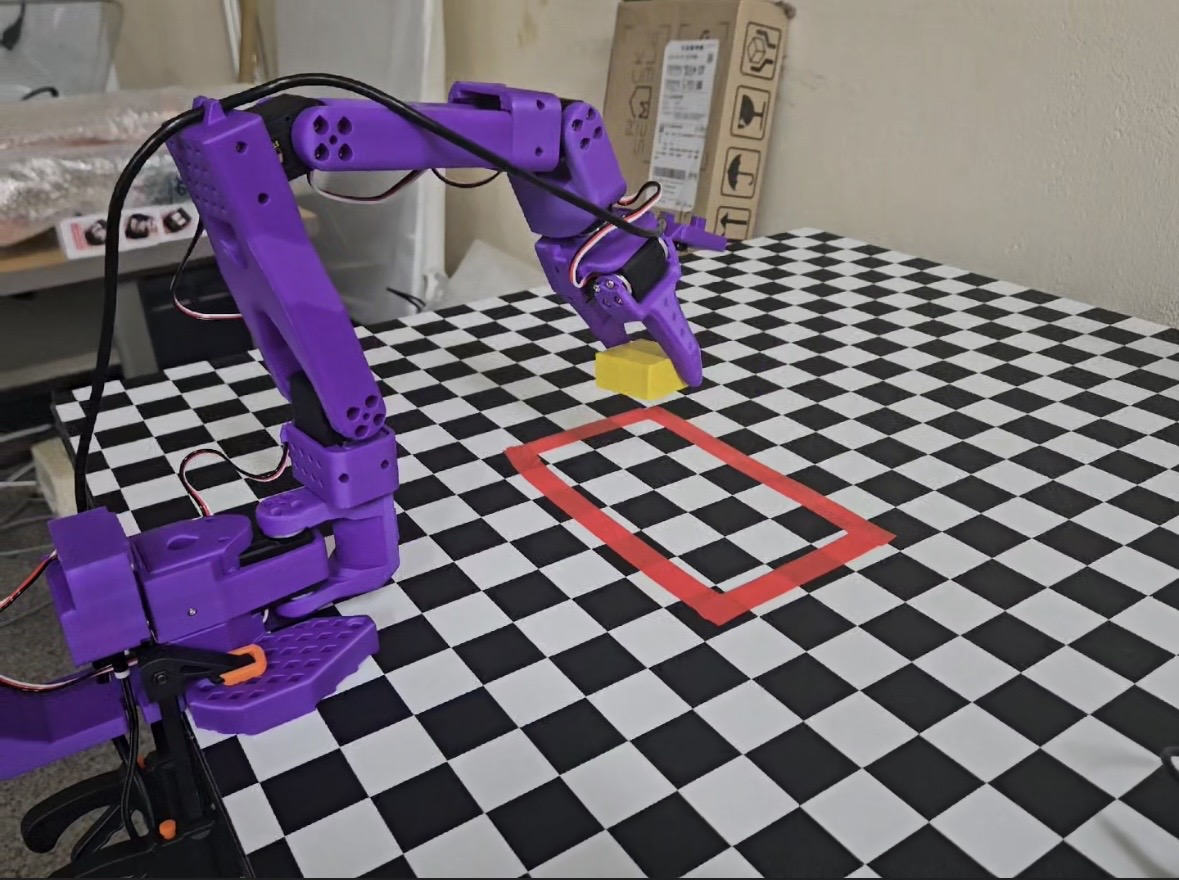
\includegraphics[width=0.6\textwidth]{grasp.png}
\caption{일반 ACT 정책이 노란 블록을 파지하여 들어 올리는 순간(1차 미션 pick-and-place 동작).}
\label{fig:result}
\end{figure}

\section{추론 및 통신 구조 검증}

데스크톱(\texttt{policy\_server})과 로봇(\texttt{robot\_client})을 gRPC로 연결하는 비동기 추론 구조를 검증하였다. Tailscale 기반 원격 환경에서 데스크톱과 Orin Nano 사이의 평균 네트워크 지연은 33ms로 측정되었다. 데스크톱 CPU만 사용한 정책 서버에서 ACT와 SmolVLA의 액션 청크 생성 시간을 측정한 결과는 표~\ref{tab:inference-time}과 같다.

\begin{longtable}{p{0.30\linewidth}p{0.22\linewidth}p{0.38\linewidth}}
\caption{데스크톱 CPU 추론 및 통신 실측 결과}\label{tab:inference-time}\\
\toprule
측정 항목 & 측정값 & 측정 조건 \\
\midrule
\endfirsthead
\toprule
측정 항목 & 측정값 & 측정 조건 \\
\midrule
\endhead
네트워크 지연 & 33ms & 데스크톱--Orin Nano 원격 연결 \\
ACT 청크 추론 & 169ms & 데스크톱 CPU, 50 actions \\
SmolVLA 청크 추론 & 879ms & 데스크톱 CPU, 50 actions \\
청크 실행 시간 & 약 1.67초 & 50 actions, 30Hz 제어 \\
\bottomrule
\end{longtable}

\begin{figure}[htbp]
\centering
\resizebox{0.96\textwidth}{!}{%
\begin{tikzpicture}[
    actor/.style   ={rectangle, rounded corners=2pt, draw=black, thick, align=center, minimum width=3.0cm, minimum height=0.9cm, font=\sffamily\small},
    note/.style    ={rectangle, draw=black!30, fill=black!4, rounded corners=1.5pt, align=left, inner sep=3.5pt, font=\sffamily\scriptsize},
    msg/.style     ={-{Latex[length=2.4mm]}, thick},
    lifeline/.style={dashed, black!50, thick},
    mlabel/.style  ={above, font=\sffamily\scriptsize, inner sep=2.5pt},
    snum/.style    ={circle, draw=black!75, fill=white, thick, inner sep=0pt, minimum size=3.9mm, font=\sffamily\scriptsize\bfseries},
    brace/.style   ={decorate, decoration={brace, amplitude=5pt}, black!60, thick}
]
\def\ox{2.0}\def\dx{10.4}
% --- overlap highlight band (drawn first, behind everything) ---
\fill[boxorange, opacity=0.6] (\ox-0.1,-5.05) rectangle (\dx+3.9,-6.05);
% --- actors and lifelines ---
\node[actor, fill=boxgreen] (orin)    at (\ox,0) {Orin Nano\\\texttt{robot\_client}};
\node[actor, fill=boxblue]  (desktop) at (\dx,0) {Desktop\\\texttt{policy\_server}};
\draw[lifeline] (orin.south)    -- (\ox,-8.6);
\draw[lifeline] (desktop.south) -- (\dx,-8.6);

% ============ initial round ============
% (1) observation -> server
\draw[msg] (\ox,-1.5) -- node[mlabel]{Observation} (\dx-0.16,-1.5);
\node[snum] at (\ox+0.75,-1.5) {1};
\node[note, anchor=north] at ({(\ox+\dx)/2},-1.72) {gRPC / Tailscale $\cdot$ 측정 네트워크 지연 33 ms};
% server inference (activation bar)
\draw[fill=boxblue, draw=black!55] (\dx-0.16,-1.95) rectangle (\dx+0.16,-3.0);
\node[note, anchor=west] at (\dx+0.55,-2.475) {추론 (50-action chunk)\\ACT 169 ms $\cdot$ SmolVLA 879 ms};
% (2) action chunk -> robot
\draw[msg] (\dx-0.16,-3.1) -- node[mlabel]{Action chunk (50 actions)} (\ox,-3.1);
\node[snum] at (\dx-0.75,-3.1) {2};

% robot executes current chunk (long activation bar)
\draw[fill=boxgreen, draw=black!55] (\ox-0.16,-3.4) rectangle (\ox+0.16,-8.2);
\draw[brace] (\ox-0.32,-3.4) -- (\ox-0.32,-8.2);
\node[anchor=east, align=right, font=\sffamily\scriptsize] at (\ox-0.5,-5.8) {현재 청크 실행\\30 Hz $\cdot$ 약 1.67 s};

% ============ overlapped round (executes while server infers) ============
% (3) next observation sent before queue depletes
\draw[msg] (\ox+0.16,-4.55) -- node[mlabel]{Next observation} (\dx-0.16,-4.55);
\node[snum] at (\ox+0.9,-4.55) {3};
% server prepares next chunk (inside overlap band)
\draw[fill=boxblue, draw=black!55] (\dx-0.16,-5.05) rectangle (\dx+0.16,-6.05);
\node[note, anchor=west] at (\dx+0.55,-5.55) {다음 청크 준비\\현재 실행과 병렬 추론};
% (4) next chunk arrives before current chunk depletes
\draw[msg] (\dx-0.16,-6.15) -- node[mlabel]{Next action chunk} (\ox+0.16,-6.15);
\node[snum] at (\dx-0.9,-6.15) {4};
% queued-ahead brace on robot side
\draw[decorate, decoration={brace, amplitude=4pt, mirror}, black!45, thick] (\ox+0.32,-6.2) -- (\ox+0.32,-8.15);
\node[anchor=west, align=left, font=\sffamily\scriptsize, text=black!70] at (\ox+0.5,-7.175) {새 청크를 큐에 적재\\제어 끊김 없이 이어짐};
\end{tikzpicture}%
}
\caption{gRPC 기반 비동기 추론 및 액션 청크 실행 시퀀스. 초기 라운드(①~②)로 첫 청크를 실행한 뒤, 현재 청크를 실행하는 동안(③) 다음 관측을 전송하여 서버가 병렬로 다음 청크를 준비한다(주황 음영). 새 청크는 현재 청크가 고갈되기 전에 도착(④)하므로 제어 끊김 없이 이어진다.}
\label{fig:async-inference-sequence}
\end{figure}

한 번의 추론으로 생성하는 50개 액션은 30Hz 제어에서 약 1.67초의 동작에 해당한다. ACT의 169ms와 SmolVLA의 879ms는 모두 이 청크 실행 시간보다 짧으므로, 현재 CPU 구성에서도 다음 청크를 실행 전에 생성할 수 있는 연산 성능을 확인하였다. 향후 GPU 옵션을 적용하여 추론 시간을 다시 측정하고, 평균값뿐 아니라 최대 지연, 액션 큐 고갈과 연속 rollout 중 제어 끊김 여부를 함께 검증한다.

\section{잔여 과제 및 후속 검증 계획}

현재까지 수집, 학습과 원격 추론의 기본 파이프라인을 확보하였으며, 이후에는 환경 변경에 따른 데이터 정비, 정책 후보 비교, 하이브리드 제어 구현과 실행 안정성 검증을 순차적으로 진행한다. 각 과제의 현재 상태와 완료 기준은 표~\ref{tab:next-steps}와 같다.

\begin{longtable}{@{}p{0.20\linewidth}p{0.39\linewidth}p{0.33\linewidth}@{}}
\caption{잔여 과제 및 후속 검증 계획}\label{tab:next-steps}\\
\toprule
과제 & 현재 상태 & 후속 검증 기준 \\
\midrule
\endfirsthead
\toprule
과제 & 현재 상태 & 후속 검증 기준 \\
\midrule
\endhead
실험 환경과 데이터 정비 & 카메라 높이와 지정구역 테이프 배치가 변경되어 새 환경 기준의 데이터가 필요하다. 색상과 초기 위치 다양성, 느린 접근과 정렬 시연을 보강하고 빨간 블록의 경계선 방향 이동 원인을 확인한다. & 새 환경 기준의 수집 조건을 확정하고, 정책 학습에 사용할 데이터셋을 재구축한다. \\
\addlinespace
정책 후보 비교 & 일반 ACT와 SmolVLA의 초기 rollout을 수행하였다. Task ID 기반 ACT와 하이브리드 ACT--CV/IK는 동일 조건 비교가 남아 있다. & 동일 초기 위치에서 반복 rollout을 수행하여 미션별 성공률, 실패 단계, 수행 시간과 추가 데이터 또는 보정 부담을 기록한다. \\
\addlinespace
하이브리드 CV/IK 검증 & HSV 기반 블록 검출, homography 좌표 변환, 비중첩 배치 슬롯과 IK 이동의 구현 및 ACT 전환 조건 검증이 필요하다. & CV 목표 좌표 오차, IK 배치 오차, ACT에서 CV/IK로의 전환 성공 여부를 측정한다. \\
\addlinespace
원격 추론 안정성 및 배포 & gRPC 기반 원격 추론과 CPU 기준 액션 청크 시간을 측정하였다. GPU 적용 성능과 장시간 실행 안정성, Docker 기반 평가 환경 호환성은 추가 확인이 필요하다. & GPU 적용 후 추론 시간, 최대 네트워크 지연, 액션 큐 고갈과 연속 rollout 중 제어 끊김 여부를 점검하고 평가 환경에서 정책 서버를 실행한다. \\
\bottomrule
\end{longtable}

환경과 데이터 정비를 먼저 완료한 뒤 정책 후보 비교와 하이브리드 제어 구현을 병행한다. 이후 비교 결과로 최종 후보를 정하고, 해당 후보에 대해 원격 실행 안정성과 평가 환경 호환성을 검증한다.

% =====================================================================
\begin{thebibliography}{99}

\bibitem{zhao2023act}
T. Z. Zhao, V. Kumar, S. Levine, and C. Finn,
\textit{Learning Fine-Grained Bimanual Manipulation with Low-Cost Hardware}, Robotics: Science and Systems (RSS), 2023. arXiv:2304.13705.

\bibitem{lerobot}
R. Cadene et al.,
\textit{LeRobot: State-of-the-art Machine Learning for Real-World Robotics in PyTorch}, Hugging Face.
Available: \url{https://github.com/huggingface/lerobot}

\bibitem{lerobot-tutorial}
Hugging Face,
\textit{Imitation Learning on Real-World Robots}, LeRobot Documentation.
Available: \url{https://huggingface.co/docs/lerobot/il_robots}

\bibitem{soarm100}
The Robot Studio,
\textit{SO-ARM100 / SO-ARM101: Standard Open Arm}, Open-Source Robot Arm Hardware.
Available: \url{https://github.com/TheRobotStudio/SO-ARM100}

\bibitem{lerobot-so101}
Hugging Face,
\textit{SO-101 Robot Arm Setup and Calibration}, LeRobot Documentation.
Available: \url{https://huggingface.co/docs/lerobot/so101}

\bibitem{lerobot-async}
Hugging Face,
\textit{Asynchronous Inference: Decoupling Action Prediction and Execution}, LeRobot Documentation.
Available: \url{https://huggingface.co/docs/lerobot/async}

\bibitem{smolvla}
M. Shukor et al.,
\textit{SmolVLA: A Vision-Language-Action Model for Affordable and Efficient Robotics}, 2025. arXiv:2506.01844.

\bibitem{opencv}
OpenCV Team,
\textit{OpenCV: Open Source Computer Vision Library}, OpenCV Documentation.
Available: \url{https://docs.opencv.org/4.x/}

\bibitem{lerobot-sim2real}
S. Tao,
\textit{LeRobot-Sim2Real: Train in Fast Simulation and Deploy Visual Policies Zero-Shot to the Real World}.
Available: \url{https://github.com/StoneT2000/lerobot-sim2real}

\bibitem{maniskill3}
S. Tao et al.,
\textit{ManiSkill3: GPU Parallelized Robotics Simulation and Rendering for Generalizable Embodied AI}, 2024. arXiv:2410.00425.

\bibitem{nvidia-jetson-orin}
NVIDIA,
\textit{Jetson Orin Nano Series Modules Data Sheet}, NVIDIA Embedded Systems Documentation.
Available: \url{https://developer.nvidia.com/embedded/downloads}

\bibitem{nvidia-tensorrt}
NVIDIA,
\textit{NVIDIA TensorRT Documentation}, Deep Learning Inference Optimizer and Runtime.
Available: \url{https://docs.nvidia.com/deeplearning/tensorrt/}

\end{thebibliography}

\end{document}
